\documentclass[twoside]{book}

% Packages required by doxygen
\usepackage{calc}
\usepackage{doxygen}
\usepackage{graphicx}
\usepackage[utf8]{inputenc}
\usepackage{makeidx}
\usepackage{multicol}
\usepackage{multirow}
\usepackage{textcomp}
\usepackage[table]{xcolor}

% NLS support packages
\usepackage{polski}
\usepackage[T1]{fontenc}

% Font selection
\usepackage[T1]{fontenc}
\usepackage{mathptmx}
\usepackage[scaled=.90]{helvet}
\usepackage{courier}
\usepackage{amssymb}
\usepackage{sectsty}
\renewcommand{\familydefault}{\sfdefault}
\allsectionsfont{%
  \fontseries{bc}\selectfont%
  \color{darkgray}%
}
\renewcommand{\DoxyLabelFont}{%
  \fontseries{bc}\selectfont%
  \color{darkgray}%
}

% Page & text layout
\usepackage{geometry}
\geometry{%
  a4paper,%
  top=2.5cm,%
  bottom=2.5cm,%
  left=2.5cm,%
  right=2.5cm%
}
\tolerance=750
\hfuzz=15pt
\hbadness=750
\setlength{\emergencystretch}{15pt}
\setlength{\parindent}{0cm}
\setlength{\parskip}{0.2cm}
\makeatletter
\renewcommand{\paragraph}{%
  \@startsection{paragraph}{4}{0ex}{-1.0ex}{1.0ex}{%
    \normalfont\normalsize\bfseries\SS@parafont%
  }%
}
\renewcommand{\subparagraph}{%
  \@startsection{subparagraph}{5}{0ex}{-1.0ex}{1.0ex}{%
    \normalfont\normalsize\bfseries\SS@subparafont%
  }%
}
\makeatother

% Headers & footers
\usepackage{fancyhdr}
\pagestyle{fancyplain}
\fancyhead[LE]{\fancyplain{}{\bfseries\thepage}}
\fancyhead[CE]{\fancyplain{}{}}
\fancyhead[RE]{\fancyplain{}{\bfseries\leftmark}}
\fancyhead[LO]{\fancyplain{}{\bfseries\rightmark}}
\fancyhead[CO]{\fancyplain{}{}}
\fancyhead[RO]{\fancyplain{}{\bfseries\thepage}}
\fancyfoot[LE]{\fancyplain{}{}}
\fancyfoot[CE]{\fancyplain{}{}}
\fancyfoot[RE]{\fancyplain{}{\bfseries\scriptsize Wygenerowano Cz, 26 mar 2015 11\-:49\-:23 dla Test struktur danych programem Doxygen }}
\fancyfoot[LO]{\fancyplain{}{\bfseries\scriptsize Wygenerowano Cz, 26 mar 2015 11\-:49\-:23 dla Test struktur danych programem Doxygen }}
\fancyfoot[CO]{\fancyplain{}{}}
\fancyfoot[RO]{\fancyplain{}{}}
\renewcommand{\footrulewidth}{0.4pt}
\renewcommand{\chaptermark}[1]{%
  \markboth{#1}{}%
}
\renewcommand{\sectionmark}[1]{%
  \markright{\thesection\ #1}%
}

% Indices & bibliography
\usepackage{natbib}
\usepackage[titles]{tocloft}
\setcounter{tocdepth}{3}
\setcounter{secnumdepth}{5}
\makeindex

% Hyperlinks (required, but should be loaded last)
\usepackage{ifpdf}
\ifpdf
  \usepackage[pdftex,pagebackref=true]{hyperref}
\else
  \usepackage[ps2pdf,pagebackref=true]{hyperref}
\fi
\hypersetup{%
  colorlinks=true,%
  linkcolor=blue,%
  citecolor=blue,%
  unicode%
}

% Custom commands
\newcommand{\clearemptydoublepage}{%
  \newpage{\pagestyle{empty}\cleardoublepage}%
}


%===== C O N T E N T S =====

\begin{document}

% Titlepage & ToC
\hypersetup{pageanchor=false}
\pagenumbering{roman}
\begin{titlepage}
\vspace*{7cm}
\begin{center}%
{\Large Test struktur danych }\\
\vspace*{1cm}
{\large Wygenerowano przez Doxygen 1.8.6}\\
\vspace*{0.5cm}
{\small Cz, 26 mar 2015 11:49:23}\\
\end{center}
\end{titlepage}
\clearemptydoublepage
\tableofcontents
\clearemptydoublepage
\pagenumbering{arabic}
\hypersetup{pageanchor=true}

%--- Begin generated contents ---
\chapter{Strona główna}
\label{index}\hypertarget{index}{}Czas wykonywania algorytmu wykonującego dodawanie elementów do podatawowych struktour danych

Program realizuje operacje dodawania n liczby elementów do listy, kolejki i stosu i mierzy czas tych operacji

\begin{DoxyAuthor}{Autor}
Mateusz Bencer
\end{DoxyAuthor}
\begin{DoxyDate}{Data}
2015.\-03.\-19
\end{DoxyDate}
\begin{DoxyVersion}{Wersja}
1.\-0
\end{DoxyVersion}
\begin{DoxyParagraph}{}
Mail\-:
\end{DoxyParagraph}
{\itshape \href{mailto:209360@pwr.wroc.edu.pl}{\tt 209360@pwr.\-wroc.\-edu.\-pl}} 

 
 \newpage
  \begin{flushleft}
test
\end{flushleft}
  
\chapter{Indeks hierarchiczny}
\section{Hierarchia klas}
Ta lista dziedziczenia posortowana jest z grubsza, choć nie całkowicie, alfabetycznie\-:\begin{DoxyCompactList}
\item \contentsline{section}{Benchmark$<$ T $>$}{\pageref{class_benchmark}}{}
\item \contentsline{section}{Element$<$ T $>$}{\pageref{class_element}}{}
\item \contentsline{section}{Array\-Implementation\-:\-:List$<$ T $>$}{\pageref{class_array_implementation_1_1_list}}{}
\item \contentsline{section}{List\-Implementation\-:\-:List$<$ T $>$}{\pageref{class_list_implementation_1_1_list}}{}
\begin{DoxyCompactList}
\item \contentsline{section}{List\-Implementation\-:\-:Queue$<$ T $>$}{\pageref{class_list_implementation_1_1_queue}}{}
\item \contentsline{section}{List\-Implementation\-:\-:Stack$<$ T $>$}{\pageref{class_list_implementation_1_1_stack}}{}
\end{DoxyCompactList}
\item \contentsline{section}{Array\-Implementation\-:\-:Queue$<$ T $>$}{\pageref{class_array_implementation_1_1_queue}}{}
\item \contentsline{section}{Array\-Implementation\-:\-:Stack$<$ T $>$}{\pageref{class_array_implementation_1_1_stack}}{}
\item \contentsline{section}{Timer}{\pageref{class_timer}}{}
\end{DoxyCompactList}

\chapter{Indeks klas}
\section{Lista klas}
Tutaj znajdują się klasy, struktury, unie i interfejsy wraz z ich krótkimi opisami\-:\begin{DoxyCompactList}
\item\contentsline{section}{\hyperlink{class_benchmark}{Benchmark$<$ T $>$} }{\pageref{class_benchmark}}{}
\item\contentsline{section}{\hyperlink{class_element}{Element$<$ T $>$} \\*Klasa reprezentująca abstrakcyjny \char`\"{}pojemnik na dane\char`\"{} }{\pageref{class_element}}{}
\item\contentsline{section}{\hyperlink{class_array_implementation_1_1_list}{Array\-Implementation\-::\-List$<$ T $>$} \\*Klasa reprezentująca podstawy konterner danych -\/ Listę zaimplementowaną na tablicy }{\pageref{class_array_implementation_1_1_list}}{}
\item\contentsline{section}{\hyperlink{class_list_implementation_1_1_list}{List\-Implementation\-::\-List$<$ T $>$} \\*Klasa reprezentująca podstawy konterner danych z którego korzystają inne -\/ Listę }{\pageref{class_list_implementation_1_1_list}}{}
\item\contentsline{section}{\hyperlink{class_array_implementation_1_1_queue}{Array\-Implementation\-::\-Queue$<$ T $>$} \\*Klasa reprezentująca podstawy konterner danych kolejke zaimplementowaną na tablicy }{\pageref{class_array_implementation_1_1_queue}}{}
\item\contentsline{section}{\hyperlink{class_list_implementation_1_1_queue}{List\-Implementation\-::\-Queue$<$ T $>$} \\*Klasa reprezentująca podstawy konterner danych kolejke }{\pageref{class_list_implementation_1_1_queue}}{}
\item\contentsline{section}{\hyperlink{class_list_implementation_1_1_stack}{List\-Implementation\-::\-Stack$<$ T $>$} \\*Klasa reprezentująca podstawy konterner danych -\/ stos }{\pageref{class_list_implementation_1_1_stack}}{}
\item\contentsline{section}{\hyperlink{class_array_implementation_1_1_stack}{Array\-Implementation\-::\-Stack$<$ T $>$} \\*Klasa reprezentująca podstawy konterner danych -\/ stos w implementacji tablicowej }{\pageref{class_array_implementation_1_1_stack}}{}
\item\contentsline{section}{\hyperlink{class_timer}{Timer} \\*Klasa do pomiaru różnicy czasów }{\pageref{class_timer}}{}
\end{DoxyCompactList}

\chapter{Indeks plików}
\section{Lista plików}
Tutaj znajduje się lista wszystkich udokumentowanych plików z ich krótkimi opisami\-:\begin{DoxyCompactList}
\item\contentsline{section}{inc/{\bfseries Benchmark.\-h} }{\pageref{_benchmark_8h}}{}
\item\contentsline{section}{inc/\hyperlink{_element_8h}{Element.\-h} \\*Deklaracja i definicja klasy \hyperlink{class_element}{Element} }{\pageref{_element_8h}}{}
\item\contentsline{section}{inc/\hyperlink{_timer_8h}{Timer.\-h} \\*Plik zawierający deklaracje klasy \hyperlink{class_timer}{Timer} służącej do pomiaru różnicy czasów }{\pageref{_timer_8h}}{}
\item\contentsline{section}{inc/\-Array\-Implementation/{\bfseries Increase.\-h} }{\pageref{_increase_8h}}{}
\item\contentsline{section}{inc/\-Array\-Implementation/\hyperlink{_array_implementation_2_list_8h}{List.\-h} \\*Deklaracja klasy Lista (w implementacji opartej na tablicy) }{\pageref{_array_implementation_2_list_8h}}{}
\item\contentsline{section}{inc/\-Array\-Implementation/\hyperlink{_array_implementation_2_queue_8h}{Queue.\-h} \\*Deklaracja i definicja klasy Queue }{\pageref{_array_implementation_2_queue_8h}}{}
\item\contentsline{section}{inc/\-Array\-Implementation/\hyperlink{_array_implementation_2_stack_8h}{Stack.\-h} \\*Deklaracja i definicja klasy Stack w wersji tablicowej }{\pageref{_array_implementation_2_stack_8h}}{}
\item\contentsline{section}{inc/\-Linked\-List\-Implementation/\hyperlink{_linked_list_implementation_2_list_8h}{List.\-h} \\*Deklaracja klasy List }{\pageref{_linked_list_implementation_2_list_8h}}{}
\item\contentsline{section}{inc/\-Linked\-List\-Implementation/\hyperlink{_linked_list_implementation_2_queue_8h}{Queue.\-h} \\*Deklaracja i definicja klasy Queue }{\pageref{_linked_list_implementation_2_queue_8h}}{}
\item\contentsline{section}{inc/\-Linked\-List\-Implementation/\hyperlink{_linked_list_implementation_2_stack_8h}{Stack.\-h} \\*Deklaracja i definicja klasy Stack }{\pageref{_linked_list_implementation_2_stack_8h}}{}
\item\contentsline{section}{src/\hyperlink{main_8cpp}{main.\-cpp} \\*Plik zawierający sekwencje operacji do mierzenia czasu operacji mnożenia elementów tablicy przez 2 }{\pageref{main_8cpp}}{}
\item\contentsline{section}{src/\hyperlink{_timer_8cpp}{Timer.\-cpp} \\*Plik zawierający definicje funkcji klasy \hyperlink{class_timer}{Timer} służącej do pomiaru różnicy czasów }{\pageref{_timer_8cpp}}{}
\end{DoxyCompactList}

\chapter{Dokumentacja klas}
\hypertarget{class_benchmark}{\section{Dokumentacja szablonu klasy Benchmark$<$ T $>$}
\label{class_benchmark}\index{Benchmark$<$ T $>$@{Benchmark$<$ T $>$}}
}
\subsection*{Metody publiczne}
\begin{DoxyCompactItemize}
\item 
\hypertarget{class_benchmark_a4b97a87100461fbeb673bb41127de761}{{\bfseries Benchmark} (unsigned int test\-Power)}\label{class_benchmark_a4b97a87100461fbeb673bb41127de761}

\item 
\hypertarget{class_benchmark_a85a0c6c3181ccbb94f4a5ee46d75d516}{void {\bfseries test\-List} (\hyperlink{class_array_implementation_1_1_list}{Array\-Implementation\-::\-List}$<$ T $>$ $\ast$list, Array\-Implementation\-::\-Increase inc)}\label{class_benchmark_a85a0c6c3181ccbb94f4a5ee46d75d516}

\item 
\hypertarget{class_benchmark_a1087f4569187951c93df6e1faed7fa49}{void {\bfseries test\-Queue} (\hyperlink{class_array_implementation_1_1_queue}{Array\-Implementation\-::\-Queue}$<$ T $>$ $\ast$queue, Array\-Implementation\-::\-Increase inc)}\label{class_benchmark_a1087f4569187951c93df6e1faed7fa49}

\item 
\hypertarget{class_benchmark_a365d3ec0d2cc52dc8e3a9dbb8c4a6a06}{void {\bfseries test\-Stack} (\hyperlink{class_array_implementation_1_1_stack}{Array\-Implementation\-::\-Stack}$<$ T $>$ $\ast$stack, Array\-Implementation\-::\-Increase inc)}\label{class_benchmark_a365d3ec0d2cc52dc8e3a9dbb8c4a6a06}

\item 
\hypertarget{class_benchmark_ad7a4484405fe92bc1c0b91ae170cd847}{void {\bfseries test\-List} (\hyperlink{class_list_implementation_1_1_list}{List\-Implementation\-::\-List}$<$ T $>$ $\ast$list)}\label{class_benchmark_ad7a4484405fe92bc1c0b91ae170cd847}

\item 
\hypertarget{class_benchmark_a3951cc83b8a85da5fd31b6bb7ca647e6}{void {\bfseries test\-Queue} (\hyperlink{class_list_implementation_1_1_queue}{List\-Implementation\-::\-Queue}$<$ T $>$ $\ast$queue)}\label{class_benchmark_a3951cc83b8a85da5fd31b6bb7ca647e6}

\item 
\hypertarget{class_benchmark_a75a11f1d9d4807e96cfa52673affa299}{void {\bfseries test\-Stack} (\hyperlink{class_list_implementation_1_1_stack}{List\-Implementation\-::\-Stack}$<$ T $>$ $\ast$stack)}\label{class_benchmark_a75a11f1d9d4807e96cfa52673affa299}

\end{DoxyCompactItemize}


Dokumentacja dla tej klasy została wygenerowana z pliku\-:\begin{DoxyCompactItemize}
\item 
inc/Benchmark.\-h\end{DoxyCompactItemize}

\hypertarget{class_element}{\section{Dokumentacja szablonu klasy Element$<$ T $>$}
\label{class_element}\index{Element$<$ T $>$@{Element$<$ T $>$}}
}


Klasa reprezentująca abstrakcyjny \char`\"{}pojemnik na dane\char`\"{}.  




{\ttfamily \#include $<$Element.\-h$>$}

\subsection*{Metody publiczne}
\begin{DoxyCompactItemize}
\item 
\hyperlink{class_element_a8d1616b3955f2039f3da1a205155e28f}{Element} (T $\ast$data)
\begin{DoxyCompactList}\small\item\em Konstruktor zapamiętujący adres przechowywanego obiektu. \end{DoxyCompactList}\item 
void \hyperlink{class_element_a60f83f9357c3266559bc6c234b5bf664}{set\-Data} (const T $\ast$data)
\begin{DoxyCompactList}\small\item\em setter do przechowywanej danej \end{DoxyCompactList}\item 
T $\ast$ \hyperlink{class_element_a3ca1fd83364406ea6928590537101d8d}{get\-Data} () const 
\begin{DoxyCompactList}\small\item\em getter do przechowywanej danej \end{DoxyCompactList}\item 
\hyperlink{class_element}{Element}$<$ T $>$ $\ast$ \hyperlink{class_element_ab37531c0ee3bcb3eeeea7f840e3df06a}{next} () const 
\begin{DoxyCompactList}\small\item\em zwraca wskaźnik do kolejnego elementu na liście \end{DoxyCompactList}\item 
\hyperlink{class_element}{Element}$<$ T $>$ $\ast$ \hyperlink{class_element_a3fee6e442312fb97eafb813e973b0001}{prev} () const 
\begin{DoxyCompactList}\small\item\em zwraca wskaźnik do poprzedniego elementu na liście \end{DoxyCompactList}\item 
void \hyperlink{class_element_abef5eda7c1de337f65fd7e021972e4a4}{set\-Next} (\hyperlink{class_element}{Element}$<$ T $>$ $\ast$\hyperlink{class_element_ab37531c0ee3bcb3eeeea7f840e3df06a}{next})
\begin{DoxyCompactList}\small\item\em ustawia kolejny element listy \end{DoxyCompactList}\item 
void \hyperlink{class_element_a8be274e88ceb7bf10f42a9880283da38}{set\-Prev} (\hyperlink{class_element}{Element}$<$ T $>$ $\ast$\hyperlink{class_element_a3fee6e442312fb97eafb813e973b0001}{prev})
\begin{DoxyCompactList}\small\item\em ustawia poprzedni element listy \end{DoxyCompactList}\item 
\hyperlink{class_element_a6d70e2988f89ccea0664dc396a05f4ab}{$\sim$\-Element} ()
\begin{DoxyCompactList}\small\item\em zwalnianie elementu przechowywanego przez klase \hyperlink{class_element}{Element} \end{DoxyCompactList}\end{DoxyCompactItemize}


\subsection{Opis szczegółowy}
\subsubsection*{template$<$class T$>$class Element$<$ T $>$}

Klasa reprezentująca abstrakcyjny \char`\"{}pojemnik na dane\char`\"{}. 

Klasa może przechowywać dane zdeterminowane przez typ szablonu, zawiera wskaźnik do kolejnego i poprzedniego elementu (implementacja elementu listy). 

\subsection{Dokumentacja konstruktora i destruktora}
\hypertarget{class_element_a8d1616b3955f2039f3da1a205155e28f}{\index{Element@{Element}!Element@{Element}}
\index{Element@{Element}!Element@{Element}}
\subsubsection[{Element}]{\setlength{\rightskip}{0pt plus 5cm}template$<$typename T $>$ {\bf Element}$<$ T $>$\-::{\bf Element} (
\begin{DoxyParamCaption}
\item[{T $\ast$}]{data}
\end{DoxyParamCaption}
)}}\label{class_element_a8d1616b3955f2039f3da1a205155e28f}


Konstruktor zapamiętujący adres przechowywanego obiektu. 


\begin{DoxyParams}{Parametry}
{\em data} & obiekt/zmięnna do przechowania \\
\hline
\end{DoxyParams}
\hypertarget{class_element_a6d70e2988f89ccea0664dc396a05f4ab}{\index{Element@{Element}!$\sim$\-Element@{$\sim$\-Element}}
\index{$\sim$\-Element@{$\sim$\-Element}!Element@{Element}}
\subsubsection[{$\sim$\-Element}]{\setlength{\rightskip}{0pt plus 5cm}template$<$typename T $>$ {\bf Element}$<$ T $>$\-::$\sim${\bf Element} (
\begin{DoxyParamCaption}
{}
\end{DoxyParamCaption}
)}}\label{class_element_a6d70e2988f89ccea0664dc396a05f4ab}


zwalnianie elementu przechowywanego przez klase \hyperlink{class_element}{Element} 

Destruktor zapewniający zwalnianie elementu przechowywanego przez klase \hyperlink{class_element}{Element} 

\subsection{Dokumentacja funkcji składowych}
\hypertarget{class_element_a3ca1fd83364406ea6928590537101d8d}{\index{Element@{Element}!get\-Data@{get\-Data}}
\index{get\-Data@{get\-Data}!Element@{Element}}
\subsubsection[{get\-Data}]{\setlength{\rightskip}{0pt plus 5cm}template$<$typename T $>$ T $\ast$ {\bf Element}$<$ T $>$\-::get\-Data (
\begin{DoxyParamCaption}
{}
\end{DoxyParamCaption}
) const}}\label{class_element_a3ca1fd83364406ea6928590537101d8d}


getter do przechowywanej danej 

Metoda do pobrania wskaźnka przechowywanego danej

\begin{DoxyReturn}{Zwraca}
wskaźnik do zmięnnej przechowywanej przez klase 
\end{DoxyReturn}
\hypertarget{class_element_ab37531c0ee3bcb3eeeea7f840e3df06a}{\index{Element@{Element}!next@{next}}
\index{next@{next}!Element@{Element}}
\subsubsection[{next}]{\setlength{\rightskip}{0pt plus 5cm}template$<$typename T $>$ {\bf Element}$<$ T $>$ $\ast$ {\bf Element}$<$ T $>$\-::next (
\begin{DoxyParamCaption}
{}
\end{DoxyParamCaption}
) const}}\label{class_element_ab37531c0ee3bcb3eeeea7f840e3df06a}


zwraca wskaźnik do kolejnego elementu na liście 

\begin{DoxyReturn}{Zwraca}
wskaźnik do kolejnego elementu na liście 
\end{DoxyReturn}
\hypertarget{class_element_a3fee6e442312fb97eafb813e973b0001}{\index{Element@{Element}!prev@{prev}}
\index{prev@{prev}!Element@{Element}}
\subsubsection[{prev}]{\setlength{\rightskip}{0pt plus 5cm}template$<$typename T $>$ {\bf Element}$<$ T $>$ $\ast$ {\bf Element}$<$ T $>$\-::prev (
\begin{DoxyParamCaption}
{}
\end{DoxyParamCaption}
) const}}\label{class_element_a3fee6e442312fb97eafb813e973b0001}


zwraca wskaźnik do poprzedniego elementu na liście 

\begin{DoxyReturn}{Zwraca}
wskaźnik do poprzedniego elementu na liście 
\end{DoxyReturn}
\hypertarget{class_element_a60f83f9357c3266559bc6c234b5bf664}{\index{Element@{Element}!set\-Data@{set\-Data}}
\index{set\-Data@{set\-Data}!Element@{Element}}
\subsubsection[{set\-Data}]{\setlength{\rightskip}{0pt plus 5cm}template$<$typename T $>$ void {\bf Element}$<$ T $>$\-::set\-Data (
\begin{DoxyParamCaption}
\item[{const T $\ast$}]{data}
\end{DoxyParamCaption}
)}}\label{class_element_a60f83f9357c3266559bc6c234b5bf664}


setter do przechowywanej danej 

Metoda do ustawiania danej przechowywanej przez klase

obiekt/zmięnna, która będzie przechowywana \hypertarget{class_element_abef5eda7c1de337f65fd7e021972e4a4}{\index{Element@{Element}!set\-Next@{set\-Next}}
\index{set\-Next@{set\-Next}!Element@{Element}}
\subsubsection[{set\-Next}]{\setlength{\rightskip}{0pt plus 5cm}template$<$typename T $>$ void {\bf Element}$<$ T $>$\-::set\-Next (
\begin{DoxyParamCaption}
\item[{{\bf Element}$<$ T $>$ $\ast$}]{next}
\end{DoxyParamCaption}
)}}\label{class_element_abef5eda7c1de337f65fd7e021972e4a4}


ustawia kolejny element listy 


\begin{DoxyParams}{Parametry}
{\em next} & kolejny element listy \\
\hline
\end{DoxyParams}
\hypertarget{class_element_a8be274e88ceb7bf10f42a9880283da38}{\index{Element@{Element}!set\-Prev@{set\-Prev}}
\index{set\-Prev@{set\-Prev}!Element@{Element}}
\subsubsection[{set\-Prev}]{\setlength{\rightskip}{0pt plus 5cm}template$<$typename T $>$ void {\bf Element}$<$ T $>$\-::set\-Prev (
\begin{DoxyParamCaption}
\item[{{\bf Element}$<$ T $>$ $\ast$}]{prev}
\end{DoxyParamCaption}
)}}\label{class_element_a8be274e88ceb7bf10f42a9880283da38}


ustawia poprzedni element listy 


\begin{DoxyParams}{Parametry}
{\em prev} & poprzedni element listy \\
\hline
\end{DoxyParams}


Dokumentacja dla tej klasy została wygenerowana z pliku\-:\begin{DoxyCompactItemize}
\item 
inc/\hyperlink{_element_8h}{Element.\-h}\end{DoxyCompactItemize}

\hypertarget{class_array_implementation_1_1_list}{\section{Dokumentacja szablonu klasy Array\-Implementation\-:\-:List$<$ T $>$}
\label{class_array_implementation_1_1_list}\index{Array\-Implementation\-::\-List$<$ T $>$@{Array\-Implementation\-::\-List$<$ T $>$}}
}


Klasa reprezentująca podstawy konterner danych -\/ Listę zaimplementowaną na tablicy.  




{\ttfamily \#include $<$List.\-h$>$}

\subsection*{Metody publiczne}
\begin{DoxyCompactItemize}
\item 
\hypertarget{class_array_implementation_1_1_list_a751192da0de1a1e4095a259f24ba4bb8}{\hyperlink{class_array_implementation_1_1_list_a751192da0de1a1e4095a259f24ba4bb8}{List} ()}\label{class_array_implementation_1_1_list_a751192da0de1a1e4095a259f24ba4bb8}

\begin{DoxyCompactList}\small\item\em Konstruktor zerujący aktualny rozmiar i przydzielający pamięć tablicy przechowującej dane w ilości \-\_\-\-M\-A\-X\-\_\-\-S\-I\-Z\-E. \end{DoxyCompactList}\item 
\hyperlink{class_array_implementation_1_1_list_a8e7dfb9fc4fb0fb71d9bbf23973f5699}{List} (unsigned int max\-\_\-size)
\begin{DoxyCompactList}\small\item\em Konstruktor zerujący rozmiar i przydzielający pamięć tablicy przechowującej dane w ilości określonej przez parametr max\-\_\-size. \end{DoxyCompactList}\item 
T $\ast$ \hyperlink{class_array_implementation_1_1_list_a24975f10b03e5aad6f326b29c0cfaa63}{pop} (unsigned int index)
\begin{DoxyCompactList}\small\item\em zwraca element o indeksie określonej przez parametr index (równocześnie usuwając go z listy) \end{DoxyCompactList}\item 
void \hyperlink{class_array_implementation_1_1_list_a4a058e7e1cfeaae6c690d924302e6b24}{push} (T $\ast$elem, unsigned int index, Increase inc)
\begin{DoxyCompactList}\small\item\em dodaje element o indkesie index do listy \end{DoxyCompactList}\item 
unsigned int \hyperlink{class_array_implementation_1_1_list_ae8da3221156f614925873483913d2d38}{size} ()
\begin{DoxyCompactList}\small\item\em zwraca aktualny rozmiar listy \end{DoxyCompactList}\item 
unsigned short \hyperlink{class_array_implementation_1_1_list_a8ff22bf7b90648b3cb1d8bf9ff3fec3a}{is\-Empty} ()
\begin{DoxyCompactList}\small\item\em zwraca 1, gdy lista jest pusta. 0, gdy są jakieś elementy \end{DoxyCompactList}\item 
\hyperlink{class_array_implementation_1_1_list_abf2ba8cfb1c4b2fa9fb585460702292b}{$\sim$\-List} ()
\begin{DoxyCompactList}\small\item\em destruktor czyszczący liste \end{DoxyCompactList}\end{DoxyCompactItemize}


\subsection{Opis szczegółowy}
\subsubsection*{template$<$class T$>$class Array\-Implementation\-::\-List$<$ T $>$}

Klasa reprezentująca podstawy konterner danych -\/ Listę zaimplementowaną na tablicy. 

Klasa reprezentująca podstawy kontener -\/ listę. Jest to implemetacja listy oparta na tablicy. 

\subsection{Dokumentacja konstruktora i destruktora}
\hypertarget{class_array_implementation_1_1_list_a8e7dfb9fc4fb0fb71d9bbf23973f5699}{\index{Array\-Implementation\-::\-List@{Array\-Implementation\-::\-List}!List@{List}}
\index{List@{List}!ArrayImplementation::List@{Array\-Implementation\-::\-List}}
\subsubsection[{List}]{\setlength{\rightskip}{0pt plus 5cm}template$<$typename T $>$ {\bf Array\-Implementation\-::\-List}$<$ T $>$\-::{\bf List} (
\begin{DoxyParamCaption}
\item[{unsigned int}]{max\-\_\-size}
\end{DoxyParamCaption}
)}}\label{class_array_implementation_1_1_list_a8e7dfb9fc4fb0fb71d9bbf23973f5699}


Konstruktor zerujący rozmiar i przydzielający pamięć tablicy przechowującej dane w ilości określonej przez parametr max\-\_\-size. 


\begin{DoxyParams}{Parametry}
{\em max\-\_\-size} & maksymalna liczba elementów w liście \\
\hline
\end{DoxyParams}
\hypertarget{class_array_implementation_1_1_list_abf2ba8cfb1c4b2fa9fb585460702292b}{\index{Array\-Implementation\-::\-List@{Array\-Implementation\-::\-List}!$\sim$\-List@{$\sim$\-List}}
\index{$\sim$\-List@{$\sim$\-List}!ArrayImplementation::List@{Array\-Implementation\-::\-List}}
\subsubsection[{$\sim$\-List}]{\setlength{\rightskip}{0pt plus 5cm}template$<$typename T $>$ {\bf Array\-Implementation\-::\-List}$<$ T $>$\-::$\sim${\bf List} (
\begin{DoxyParamCaption}
{}
\end{DoxyParamCaption}
)}}\label{class_array_implementation_1_1_list_abf2ba8cfb1c4b2fa9fb585460702292b}


destruktor czyszczący liste 

Destruktor usuwawa wszystkie elementy z listy 

\subsection{Dokumentacja funkcji składowych}
\hypertarget{class_array_implementation_1_1_list_a8ff22bf7b90648b3cb1d8bf9ff3fec3a}{\index{Array\-Implementation\-::\-List@{Array\-Implementation\-::\-List}!is\-Empty@{is\-Empty}}
\index{is\-Empty@{is\-Empty}!ArrayImplementation::List@{Array\-Implementation\-::\-List}}
\subsubsection[{is\-Empty}]{\setlength{\rightskip}{0pt plus 5cm}template$<$typename T $>$ unsigned short {\bf Array\-Implementation\-::\-List}$<$ T $>$\-::is\-Empty (
\begin{DoxyParamCaption}
{}
\end{DoxyParamCaption}
)}}\label{class_array_implementation_1_1_list_a8ff22bf7b90648b3cb1d8bf9ff3fec3a}


zwraca 1, gdy lista jest pusta. 0, gdy są jakieś elementy 

\begin{DoxyReturn}{Zwraca}
zwraca informacje, czy w liście są jakieś elementy 
\end{DoxyReturn}
\hypertarget{class_array_implementation_1_1_list_a24975f10b03e5aad6f326b29c0cfaa63}{\index{Array\-Implementation\-::\-List@{Array\-Implementation\-::\-List}!pop@{pop}}
\index{pop@{pop}!ArrayImplementation::List@{Array\-Implementation\-::\-List}}
\subsubsection[{pop}]{\setlength{\rightskip}{0pt plus 5cm}template$<$typename T $>$ T $\ast$ {\bf Array\-Implementation\-::\-List}$<$ T $>$\-::pop (
\begin{DoxyParamCaption}
\item[{unsigned int}]{index}
\end{DoxyParamCaption}
)}}\label{class_array_implementation_1_1_list_a24975f10b03e5aad6f326b29c0cfaa63}


zwraca element o indeksie określonej przez parametr index (równocześnie usuwając go z listy) 


\begin{DoxyParams}{Parametry}
{\em index} & określa indeks elementu znajdującego się na liście, który zostanie zwrócony \\
\hline
\end{DoxyParams}
\begin{DoxyReturn}{Zwraca}
element listy o pozycji index 
\end{DoxyReturn}
\hypertarget{class_array_implementation_1_1_list_a4a058e7e1cfeaae6c690d924302e6b24}{\index{Array\-Implementation\-::\-List@{Array\-Implementation\-::\-List}!push@{push}}
\index{push@{push}!ArrayImplementation::List@{Array\-Implementation\-::\-List}}
\subsubsection[{push}]{\setlength{\rightskip}{0pt plus 5cm}template$<$typename T $>$ void {\bf Array\-Implementation\-::\-List}$<$ T $>$\-::push (
\begin{DoxyParamCaption}
\item[{T $\ast$}]{elem, }
\item[{unsigned int}]{index, }
\item[{Increase}]{inc}
\end{DoxyParamCaption}
)}}\label{class_array_implementation_1_1_list_a4a058e7e1cfeaae6c690d924302e6b24}


dodaje element o indkesie index do listy 

\begin{DoxyPrecond}{Warunek wstępny}
Indeksowanie zaczyna się od 1 
\end{DoxyPrecond}

\begin{DoxyParams}{Parametry}
{\em elem} & element umieszczany do listy \\
\hline
{\em index} & określa pozycję na liście dodawanego elementu (numeracja od 1!) \\
\hline
{\em inc} & określa sposób powiększania się listy w razie braku miejsca \\
\hline
\end{DoxyParams}
\hypertarget{class_array_implementation_1_1_list_ae8da3221156f614925873483913d2d38}{\index{Array\-Implementation\-::\-List@{Array\-Implementation\-::\-List}!size@{size}}
\index{size@{size}!ArrayImplementation::List@{Array\-Implementation\-::\-List}}
\subsubsection[{size}]{\setlength{\rightskip}{0pt plus 5cm}template$<$typename T $>$ unsigned int {\bf Array\-Implementation\-::\-List}$<$ T $>$\-::size (
\begin{DoxyParamCaption}
{}
\end{DoxyParamCaption}
)}}\label{class_array_implementation_1_1_list_ae8da3221156f614925873483913d2d38}


zwraca aktualny rozmiar listy 

\begin{DoxyReturn}{Zwraca}
rozmiar listy 
\end{DoxyReturn}


Dokumentacja dla tej klasy została wygenerowana z pliku\-:\begin{DoxyCompactItemize}
\item 
inc/\-Array\-Implementation/\hyperlink{_array_implementation_2_list_8h}{List.\-h}\end{DoxyCompactItemize}

\hypertarget{class_list_implementation_1_1_list}{\section{Dokumentacja szablonu klasy List\-Implementation\-:\-:List$<$ T $>$}
\label{class_list_implementation_1_1_list}\index{List\-Implementation\-::\-List$<$ T $>$@{List\-Implementation\-::\-List$<$ T $>$}}
}


Klasa reprezentująca podstawy konterner danych z którego korzystają inne -\/ Listę  




{\ttfamily \#include $<$List.\-h$>$}

Diagram dziedziczenia dla List\-Implementation\-:\-:List$<$ T $>$\begin{figure}[H]
\begin{center}
\leavevmode
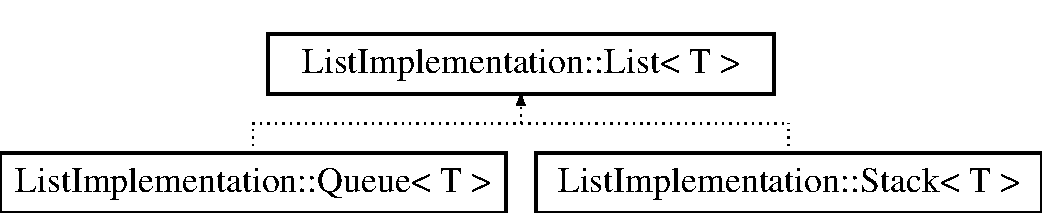
\includegraphics[height=2.000000cm]{class_list_implementation_1_1_list}
\end{center}
\end{figure}
\subsection*{Metody publiczne}
\begin{DoxyCompactItemize}
\item 
\hypertarget{class_list_implementation_1_1_list_a10d3f7ae55c6a0fecfc128adce8c780a}{\hyperlink{class_list_implementation_1_1_list_a10d3f7ae55c6a0fecfc128adce8c780a}{List} ()}\label{class_list_implementation_1_1_list_a10d3f7ae55c6a0fecfc128adce8c780a}

\begin{DoxyCompactList}\small\item\em Konstruktor zerujący pola klasy i przydzielający pamięć na \-\_\-head i \-\_\-tail. \end{DoxyCompactList}\item 
\hyperlink{class_element}{Element}$<$ T $>$ $\ast$ \hyperlink{class_list_implementation_1_1_list_ade59f70b0f166150ad68f7c21cceb6f2}{pop} (Direction dir)
\begin{DoxyCompactList}\small\item\em zwraca element z początku(zależy od użytej struktury danych) listy \end{DoxyCompactList}\item 
void \hyperlink{class_list_implementation_1_1_list_a8138a1cf63d2fa78f96225871d1e2e9d}{push} (\hyperlink{class_element}{Element}$<$ T $>$ $\ast$elem, Direction dir)
\begin{DoxyCompactList}\small\item\em dodaje element na początek/koniec(zależy od implementacji) listy \end{DoxyCompactList}\item 
unsigned int \hyperlink{class_list_implementation_1_1_list_a4478f376ab24848ed7809c3819c31dfd}{size} ()
\begin{DoxyCompactList}\small\item\em zwraca rozmiar użytej struktury danych \end{DoxyCompactList}\item 
unsigned short \hyperlink{class_list_implementation_1_1_list_a1a886e08a6c178dfe3fc0d5285672f27}{is\-Empty} ()
\begin{DoxyCompactList}\small\item\em zwraca 1, gdy kontener jest pusty, 0 -\/ gdy jest już jakiś element \end{DoxyCompactList}\item 
virtual \hyperlink{class_list_implementation_1_1_list_a6d73f9b98132a4503ffd440eb8ae2afd}{$\sim$\-List} ()
\begin{DoxyCompactList}\small\item\em wirtualny destruktor czyszczący liste \end{DoxyCompactList}\end{DoxyCompactItemize}


\subsection{Opis szczegółowy}
\subsubsection*{template$<$class T$>$class List\-Implementation\-::\-List$<$ T $>$}

Klasa reprezentująca podstawy konterner danych z którego korzystają inne -\/ Listę 

Klasa reprezentująca podstawy kontener -\/ listę. Jest to podstawowa implementacja listy stanowiąca klase bazową dla listy, stosu i kolejki 

\subsection{Dokumentacja konstruktora i destruktora}
\hypertarget{class_list_implementation_1_1_list_a6d73f9b98132a4503ffd440eb8ae2afd}{\index{List\-Implementation\-::\-List@{List\-Implementation\-::\-List}!$\sim$\-List@{$\sim$\-List}}
\index{$\sim$\-List@{$\sim$\-List}!ListImplementation::List@{List\-Implementation\-::\-List}}
\subsubsection[{$\sim$\-List}]{\setlength{\rightskip}{0pt plus 5cm}template$<$typename T $>$ {\bf List\-Implementation\-::\-List}$<$ T $>$\-::$\sim${\bf List} (
\begin{DoxyParamCaption}
{}
\end{DoxyParamCaption}
)\hspace{0.3cm}{\ttfamily [virtual]}}}\label{class_list_implementation_1_1_list_a6d73f9b98132a4503ffd440eb8ae2afd}


wirtualny destruktor czyszczący liste 

Destruktor usuwawa wszystkie elementy z listy 

\subsection{Dokumentacja funkcji składowych}
\hypertarget{class_list_implementation_1_1_list_a1a886e08a6c178dfe3fc0d5285672f27}{\index{List\-Implementation\-::\-List@{List\-Implementation\-::\-List}!is\-Empty@{is\-Empty}}
\index{is\-Empty@{is\-Empty}!ListImplementation::List@{List\-Implementation\-::\-List}}
\subsubsection[{is\-Empty}]{\setlength{\rightskip}{0pt plus 5cm}template$<$typename T $>$ unsigned short {\bf List\-Implementation\-::\-List}$<$ T $>$\-::is\-Empty (
\begin{DoxyParamCaption}
{}
\end{DoxyParamCaption}
)}}\label{class_list_implementation_1_1_list_a1a886e08a6c178dfe3fc0d5285672f27}


zwraca 1, gdy kontener jest pusty, 0 -\/ gdy jest już jakiś element 

\begin{DoxyReturn}{Zwraca}
zwraca informacje, czy w kontenerze są już jakieś elementy 
\end{DoxyReturn}
\hypertarget{class_list_implementation_1_1_list_ade59f70b0f166150ad68f7c21cceb6f2}{\index{List\-Implementation\-::\-List@{List\-Implementation\-::\-List}!pop@{pop}}
\index{pop@{pop}!ListImplementation::List@{List\-Implementation\-::\-List}}
\subsubsection[{pop}]{\setlength{\rightskip}{0pt plus 5cm}template$<$typename T $>$ {\bf Element}$<$ T $>$ $\ast$ {\bf List\-Implementation\-::\-List}$<$ T $>$\-::pop (
\begin{DoxyParamCaption}
\item[{Direction}]{dir}
\end{DoxyParamCaption}
)}}\label{class_list_implementation_1_1_list_ade59f70b0f166150ad68f7c21cceb6f2}


zwraca element z początku(zależy od użytej struktury danych) listy 


\begin{DoxyParams}{Parametry}
{\em dir} & określa czy zdjąć element z początku (Front), czy z końca (Back) listy \\
\hline
\end{DoxyParams}
\begin{DoxyReturn}{Zwraca}
element będący na początku/końcu listy 
\end{DoxyReturn}
\hypertarget{class_list_implementation_1_1_list_a8138a1cf63d2fa78f96225871d1e2e9d}{\index{List\-Implementation\-::\-List@{List\-Implementation\-::\-List}!push@{push}}
\index{push@{push}!ListImplementation::List@{List\-Implementation\-::\-List}}
\subsubsection[{push}]{\setlength{\rightskip}{0pt plus 5cm}template$<$typename T $>$ void {\bf List\-Implementation\-::\-List}$<$ T $>$\-::push (
\begin{DoxyParamCaption}
\item[{{\bf Element}$<$ T $>$ $\ast$}]{elem, }
\item[{Direction}]{dir}
\end{DoxyParamCaption}
)}}\label{class_list_implementation_1_1_list_a8138a1cf63d2fa78f96225871d1e2e9d}


dodaje element na początek/koniec(zależy od implementacji) listy 


\begin{DoxyParams}{Parametry}
{\em elem} & element umieszczany na początku/końcu listy \\
\hline
{\em dir} & określa czy włożyć element na początek(\-Front), na koniec (Back) listy \\
\hline
\end{DoxyParams}
\hypertarget{class_list_implementation_1_1_list_a4478f376ab24848ed7809c3819c31dfd}{\index{List\-Implementation\-::\-List@{List\-Implementation\-::\-List}!size@{size}}
\index{size@{size}!ListImplementation::List@{List\-Implementation\-::\-List}}
\subsubsection[{size}]{\setlength{\rightskip}{0pt plus 5cm}template$<$typename T $>$ unsigned int {\bf List\-Implementation\-::\-List}$<$ T $>$\-::size (
\begin{DoxyParamCaption}
{}
\end{DoxyParamCaption}
)}}\label{class_list_implementation_1_1_list_a4478f376ab24848ed7809c3819c31dfd}


zwraca rozmiar użytej struktury danych 

\begin{DoxyReturn}{Zwraca}
rozmiar użytej struktury danych 
\end{DoxyReturn}


Dokumentacja dla tej klasy została wygenerowana z pliku\-:\begin{DoxyCompactItemize}
\item 
inc/\-Linked\-List\-Implementation/\hyperlink{_linked_list_implementation_2_list_8h}{List.\-h}\end{DoxyCompactItemize}

\hypertarget{class_array_implementation_1_1_queue}{\section{Dokumentacja szablonu klasy Array\-Implementation\-:\-:Queue$<$ T $>$}
\label{class_array_implementation_1_1_queue}\index{Array\-Implementation\-::\-Queue$<$ T $>$@{Array\-Implementation\-::\-Queue$<$ T $>$}}
}


Klasa reprezentująca podstawy konterner danych kolejke zaimplementowaną na tablicy.  




{\ttfamily \#include $<$Queue.\-h$>$}

\subsection*{Metody publiczne}
\begin{DoxyCompactItemize}
\item 
\hypertarget{class_array_implementation_1_1_queue_ac7a57953bf0b2f661e51eebff2ce3a33}{\hyperlink{class_array_implementation_1_1_queue_ac7a57953bf0b2f661e51eebff2ce3a33}{Queue} ()}\label{class_array_implementation_1_1_queue_ac7a57953bf0b2f661e51eebff2ce3a33}

\begin{DoxyCompactList}\small\item\em Konstruktor alokujący pamięć na kolejkę oraz zerujący indeks elementu na końcu kolejki. \end{DoxyCompactList}\item 
\hyperlink{class_array_implementation_1_1_queue_ac17b065619517a4cbdd0f5b32d007548}{Queue} (unsigned int max\-\_\-size)
\begin{DoxyCompactList}\small\item\em Konstruktor alokujący pamięć na kolejkę w ilości max\-\_\-size oraz zerujący indeks elementu na końcu kolejki. \end{DoxyCompactList}\item 
T $\ast$ \hyperlink{class_array_implementation_1_1_queue_a9cb6a0e891a5bd1086028dadcadcc8c3}{pop} ()
\begin{DoxyCompactList}\small\item\em zwraca element z początku kolejki \end{DoxyCompactList}\item 
void \hyperlink{class_array_implementation_1_1_queue_afafcb7c4d247f8e887b6f29dc179bd38}{push} (T $\ast$elem, Increase inc)
\begin{DoxyCompactList}\small\item\em dodaje element na koniec kolejki \end{DoxyCompactList}\item 
\hypertarget{class_array_implementation_1_1_queue_ad178e4eee785f70f83fb9526fbaeea16}{\hyperlink{class_array_implementation_1_1_queue_ad178e4eee785f70f83fb9526fbaeea16}{$\sim$\-Queue} ()}\label{class_array_implementation_1_1_queue_ad178e4eee785f70f83fb9526fbaeea16}

\begin{DoxyCompactList}\small\item\em Destruktor usuwa tablicę przechowującą elementy kolejki. \end{DoxyCompactList}\end{DoxyCompactItemize}


\subsection{Opis szczegółowy}
\subsubsection*{template$<$class T$>$class Array\-Implementation\-::\-Queue$<$ T $>$}

Klasa reprezentująca podstawy konterner danych kolejke zaimplementowaną na tablicy. 

Kolejka jest strukturą danych typu typu F\-I\-F\-O, First In, First Out; pierwszy na wejściu, pierwszy na wyjściu 

\subsection{Dokumentacja konstruktora i destruktora}
\hypertarget{class_array_implementation_1_1_queue_ac17b065619517a4cbdd0f5b32d007548}{\index{Array\-Implementation\-::\-Queue@{Array\-Implementation\-::\-Queue}!Queue@{Queue}}
\index{Queue@{Queue}!ArrayImplementation::Queue@{Array\-Implementation\-::\-Queue}}
\subsubsection[{Queue}]{\setlength{\rightskip}{0pt plus 5cm}template$<$typename T $>$ {\bf Array\-Implementation\-::\-Queue}$<$ T $>$\-::{\bf Queue} (
\begin{DoxyParamCaption}
\item[{unsigned int}]{max\-\_\-size}
\end{DoxyParamCaption}
)}}\label{class_array_implementation_1_1_queue_ac17b065619517a4cbdd0f5b32d007548}


Konstruktor alokujący pamięć na kolejkę w ilości max\-\_\-size oraz zerujący indeks elementu na końcu kolejki. 


\begin{DoxyParams}{Parametry}
{\em max\-\_\-size} & maksymalna liczba elementów w kolejce \\
\hline
\end{DoxyParams}


\subsection{Dokumentacja funkcji składowych}
\hypertarget{class_array_implementation_1_1_queue_a9cb6a0e891a5bd1086028dadcadcc8c3}{\index{Array\-Implementation\-::\-Queue@{Array\-Implementation\-::\-Queue}!pop@{pop}}
\index{pop@{pop}!ArrayImplementation::Queue@{Array\-Implementation\-::\-Queue}}
\subsubsection[{pop}]{\setlength{\rightskip}{0pt plus 5cm}template$<$typename T $>$ T $\ast$ {\bf Array\-Implementation\-::\-Queue}$<$ T $>$\-::pop (
\begin{DoxyParamCaption}
{}
\end{DoxyParamCaption}
)}}\label{class_array_implementation_1_1_queue_a9cb6a0e891a5bd1086028dadcadcc8c3}


zwraca element z początku kolejki 

\begin{DoxyReturn}{Zwraca}
element będący na początku kolejki 
\end{DoxyReturn}
\hypertarget{class_array_implementation_1_1_queue_afafcb7c4d247f8e887b6f29dc179bd38}{\index{Array\-Implementation\-::\-Queue@{Array\-Implementation\-::\-Queue}!push@{push}}
\index{push@{push}!ArrayImplementation::Queue@{Array\-Implementation\-::\-Queue}}
\subsubsection[{push}]{\setlength{\rightskip}{0pt plus 5cm}template$<$typename T $>$ void {\bf Array\-Implementation\-::\-Queue}$<$ T $>$\-::push (
\begin{DoxyParamCaption}
\item[{T $\ast$}]{elem, }
\item[{Increase}]{inc}
\end{DoxyParamCaption}
)}}\label{class_array_implementation_1_1_queue_afafcb7c4d247f8e887b6f29dc179bd38}


dodaje element na koniec kolejki 


\begin{DoxyParams}{Parametry}
{\em elem} & element umieszczany na końcu kolejki \\
\hline
{\em inc} & określa sposób powiększania się kolejki w razie braku miejsca \\
\hline
\end{DoxyParams}


Dokumentacja dla tej klasy została wygenerowana z pliku\-:\begin{DoxyCompactItemize}
\item 
inc/\-Array\-Implementation/\hyperlink{_array_implementation_2_queue_8h}{Queue.\-h}\end{DoxyCompactItemize}

\hypertarget{class_list_implementation_1_1_queue}{\section{Dokumentacja szablonu klasy List\-Implementation\-:\-:Queue$<$ T $>$}
\label{class_list_implementation_1_1_queue}\index{List\-Implementation\-::\-Queue$<$ T $>$@{List\-Implementation\-::\-Queue$<$ T $>$}}
}


Klasa reprezentująca podstawy konterner danych kolejke.  




{\ttfamily \#include $<$Queue.\-h$>$}

Diagram dziedziczenia dla List\-Implementation\-:\-:Queue$<$ T $>$\begin{figure}[H]
\begin{center}
\leavevmode
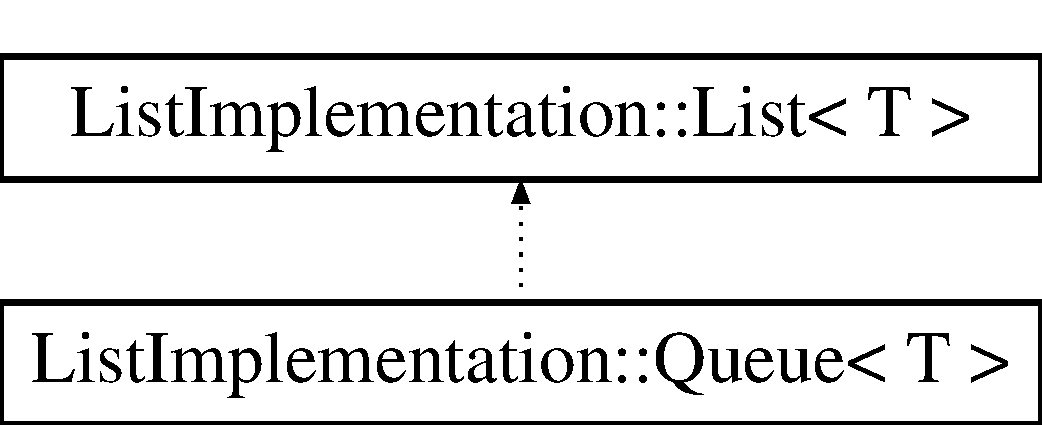
\includegraphics[height=2.000000cm]{class_list_implementation_1_1_queue}
\end{center}
\end{figure}
\subsection*{Metody publiczne}
\begin{DoxyCompactItemize}
\item 
\hypertarget{class_list_implementation_1_1_queue_acc4029f7302ff7285eb04a95617fc280}{\hyperlink{class_list_implementation_1_1_queue_acc4029f7302ff7285eb04a95617fc280}{Queue} ()}\label{class_list_implementation_1_1_queue_acc4029f7302ff7285eb04a95617fc280}

\begin{DoxyCompactList}\small\item\em Konstruktor wywołujący konstruktor klasy bazowej \hyperlink{class_list_implementation_1_1_list}{List}. \end{DoxyCompactList}\item 
\hyperlink{class_element}{Element}$<$ T $>$ $\ast$ \hyperlink{class_list_implementation_1_1_queue_a8860612212b3ab036b2032dc1ee0cb63}{pop} ()
\begin{DoxyCompactList}\small\item\em zwraca element z początku kolejki \end{DoxyCompactList}\item 
void \hyperlink{class_list_implementation_1_1_queue_a4b4439f3c97e53691620787cf2847cdc}{push} (\hyperlink{class_element}{Element}$<$ T $>$ $\ast$elem)
\begin{DoxyCompactList}\small\item\em dodaje element na koniec kolejki \end{DoxyCompactList}\item 
\hypertarget{class_list_implementation_1_1_queue_ab7c68be079c746681443aa0b06075f24}{virtual \hyperlink{class_list_implementation_1_1_queue_ab7c68be079c746681443aa0b06075f24}{$\sim$\-Queue} ()}\label{class_list_implementation_1_1_queue_ab7c68be079c746681443aa0b06075f24}

\begin{DoxyCompactList}\small\item\em Wywołuje destruktor klasy bazowej. \end{DoxyCompactList}\end{DoxyCompactItemize}


\subsection{Opis szczegółowy}
\subsubsection*{template$<$class T$>$class List\-Implementation\-::\-Queue$<$ T $>$}

Klasa reprezentująca podstawy konterner danych kolejke. 

Kolejka jest strukturą danych typu typu F\-I\-F\-O, First In, First Out; pierwszy na wejściu, pierwszy na wyjściu 

\subsection{Dokumentacja funkcji składowych}
\hypertarget{class_list_implementation_1_1_queue_a8860612212b3ab036b2032dc1ee0cb63}{\index{List\-Implementation\-::\-Queue@{List\-Implementation\-::\-Queue}!pop@{pop}}
\index{pop@{pop}!ListImplementation::Queue@{List\-Implementation\-::\-Queue}}
\subsubsection[{pop}]{\setlength{\rightskip}{0pt plus 5cm}template$<$typename T $>$ {\bf Element}$<$ T $>$ $\ast$ {\bf List\-Implementation\-::\-Queue}$<$ T $>$\-::pop (
\begin{DoxyParamCaption}
{}
\end{DoxyParamCaption}
)}}\label{class_list_implementation_1_1_queue_a8860612212b3ab036b2032dc1ee0cb63}


zwraca element z początku kolejki 

\begin{DoxyReturn}{Zwraca}
element będący na początku kolejki 
\end{DoxyReturn}
\hypertarget{class_list_implementation_1_1_queue_a4b4439f3c97e53691620787cf2847cdc}{\index{List\-Implementation\-::\-Queue@{List\-Implementation\-::\-Queue}!push@{push}}
\index{push@{push}!ListImplementation::Queue@{List\-Implementation\-::\-Queue}}
\subsubsection[{push}]{\setlength{\rightskip}{0pt plus 5cm}template$<$typename T $>$ void {\bf List\-Implementation\-::\-Queue}$<$ T $>$\-::push (
\begin{DoxyParamCaption}
\item[{{\bf Element}$<$ T $>$ $\ast$}]{elem}
\end{DoxyParamCaption}
)}}\label{class_list_implementation_1_1_queue_a4b4439f3c97e53691620787cf2847cdc}


dodaje element na koniec kolejki 


\begin{DoxyParams}{Parametry}
{\em elem} & element umieszczany na końcu \\
\hline
\end{DoxyParams}


Dokumentacja dla tej klasy została wygenerowana z pliku\-:\begin{DoxyCompactItemize}
\item 
inc/\-Linked\-List\-Implementation/\hyperlink{_linked_list_implementation_2_queue_8h}{Queue.\-h}\end{DoxyCompactItemize}

\hypertarget{class_list_implementation_1_1_stack}{\section{Dokumentacja szablonu klasy List\-Implementation\-:\-:Stack$<$ T $>$}
\label{class_list_implementation_1_1_stack}\index{List\-Implementation\-::\-Stack$<$ T $>$@{List\-Implementation\-::\-Stack$<$ T $>$}}
}


Klasa reprezentująca podstawy konterner danych -\/ stos.  




{\ttfamily \#include $<$Stack.\-h$>$}

Diagram dziedziczenia dla List\-Implementation\-:\-:Stack$<$ T $>$\begin{figure}[H]
\begin{center}
\leavevmode
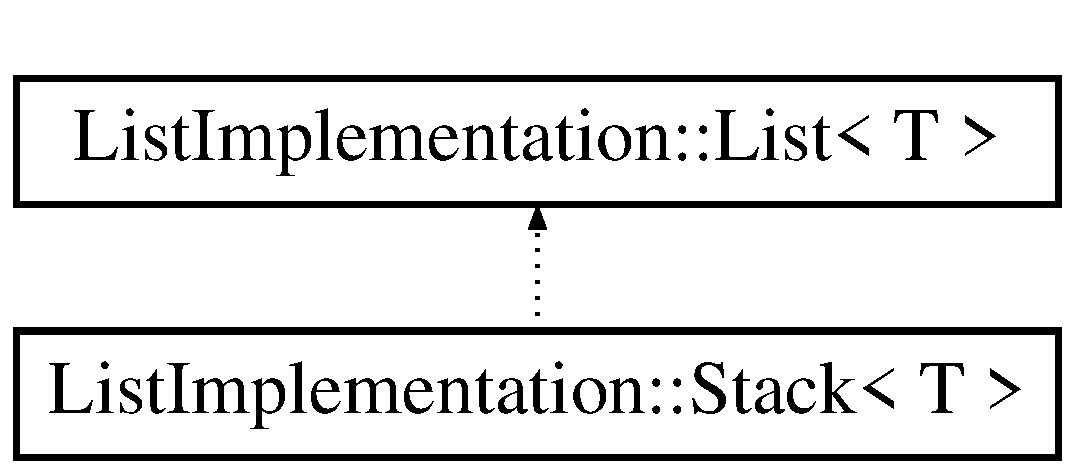
\includegraphics[height=2.000000cm]{class_list_implementation_1_1_stack}
\end{center}
\end{figure}
\subsection*{Metody publiczne}
\begin{DoxyCompactItemize}
\item 
\hypertarget{class_list_implementation_1_1_stack_adb5bbd213fc32837a8bccfe76dd40d64}{\hyperlink{class_list_implementation_1_1_stack_adb5bbd213fc32837a8bccfe76dd40d64}{Stack} ()}\label{class_list_implementation_1_1_stack_adb5bbd213fc32837a8bccfe76dd40d64}

\begin{DoxyCompactList}\small\item\em Konstruktor wywołujący konstruktor klasy bazowej \hyperlink{class_list_implementation_1_1_list}{List}. \end{DoxyCompactList}\item 
\hyperlink{class_element}{Element}$<$ T $>$ $\ast$ \hyperlink{class_list_implementation_1_1_stack_abdb24c8782d108c5860d7cdf6684edcb}{pop} ()
\begin{DoxyCompactList}\small\item\em zwraca element z wierzchu stosu \end{DoxyCompactList}\item 
void \hyperlink{class_list_implementation_1_1_stack_a68d1136b2a159ebb9a0f3f8b6556f404}{push} (\hyperlink{class_element}{Element}$<$ T $>$ $\ast$elem)
\begin{DoxyCompactList}\small\item\em dodaje element na wierzch \end{DoxyCompactList}\item 
\hypertarget{class_list_implementation_1_1_stack_a42841378ab51ccfd0e666db83daa5365}{virtual \hyperlink{class_list_implementation_1_1_stack_a42841378ab51ccfd0e666db83daa5365}{$\sim$\-Stack} ()}\label{class_list_implementation_1_1_stack_a42841378ab51ccfd0e666db83daa5365}

\begin{DoxyCompactList}\small\item\em Wywołuje destruktor klasy bazowej. \end{DoxyCompactList}\end{DoxyCompactItemize}


\subsection{Opis szczegółowy}
\subsubsection*{template$<$class T$>$class List\-Implementation\-::\-Stack$<$ T $>$}

Klasa reprezentująca podstawy konterner danych -\/ stos. 

Kolejka jest strukturą danych typu typu L\-I\-F\-O, Last In, First Out; ostatni na wejściu, pierwszy na wyjściu 

\subsection{Dokumentacja funkcji składowych}
\hypertarget{class_list_implementation_1_1_stack_abdb24c8782d108c5860d7cdf6684edcb}{\index{List\-Implementation\-::\-Stack@{List\-Implementation\-::\-Stack}!pop@{pop}}
\index{pop@{pop}!ListImplementation::Stack@{List\-Implementation\-::\-Stack}}
\subsubsection[{pop}]{\setlength{\rightskip}{0pt plus 5cm}template$<$typename T $>$ {\bf Element}$<$ T $>$ $\ast$ {\bf List\-Implementation\-::\-Stack}$<$ T $>$\-::pop (
\begin{DoxyParamCaption}
{}
\end{DoxyParamCaption}
)}}\label{class_list_implementation_1_1_stack_abdb24c8782d108c5860d7cdf6684edcb}


zwraca element z wierzchu stosu 

\begin{DoxyReturn}{Zwraca}
element będący na wierzchu stosu 
\end{DoxyReturn}
\hypertarget{class_list_implementation_1_1_stack_a68d1136b2a159ebb9a0f3f8b6556f404}{\index{List\-Implementation\-::\-Stack@{List\-Implementation\-::\-Stack}!push@{push}}
\index{push@{push}!ListImplementation::Stack@{List\-Implementation\-::\-Stack}}
\subsubsection[{push}]{\setlength{\rightskip}{0pt plus 5cm}template$<$typename T $>$ void {\bf List\-Implementation\-::\-Stack}$<$ T $>$\-::push (
\begin{DoxyParamCaption}
\item[{{\bf Element}$<$ T $>$ $\ast$}]{elem}
\end{DoxyParamCaption}
)}}\label{class_list_implementation_1_1_stack_a68d1136b2a159ebb9a0f3f8b6556f404}


dodaje element na wierzch 


\begin{DoxyParams}{Parametry}
{\em elem} & element, który zostanie umieszczony na wierzchu stosu \\
\hline
\end{DoxyParams}


Dokumentacja dla tej klasy została wygenerowana z pliku\-:\begin{DoxyCompactItemize}
\item 
inc/\-Linked\-List\-Implementation/\hyperlink{_linked_list_implementation_2_stack_8h}{Stack.\-h}\end{DoxyCompactItemize}

\hypertarget{class_array_implementation_1_1_stack}{\section{Dokumentacja szablonu klasy Array\-Implementation\-:\-:Stack$<$ T $>$}
\label{class_array_implementation_1_1_stack}\index{Array\-Implementation\-::\-Stack$<$ T $>$@{Array\-Implementation\-::\-Stack$<$ T $>$}}
}


Klasa reprezentująca podstawy konterner danych -\/ stos w implementacji tablicowej.  




{\ttfamily \#include $<$Stack.\-h$>$}

\subsection*{Metody publiczne}
\begin{DoxyCompactItemize}
\item 
\hypertarget{class_array_implementation_1_1_stack_af8a18d276411683337c92cc561a0b818}{\hyperlink{class_array_implementation_1_1_stack_af8a18d276411683337c92cc561a0b818}{Stack} ()}\label{class_array_implementation_1_1_stack_af8a18d276411683337c92cc561a0b818}

\begin{DoxyCompactList}\small\item\em Konstruktor przydzielający pamieć na stos w ilości \-\_\-\-M\-A\-X\-\_\-\-S\-I\-Z\-E oraz zerujący szczyt stosu. \end{DoxyCompactList}\item 
\hyperlink{class_array_implementation_1_1_stack_a318a54555d60ce71f4a1481c0abe6767}{Stack} (int max\-\_\-size)
\begin{DoxyCompactList}\small\item\em Konstruktor przydzielający pamieć na stos w ilości max\-\_\-size oraz zerujący szczyt stosu. \end{DoxyCompactList}\item 
\hyperlink{class_element}{Element}$<$ T $>$ $\ast$ \hyperlink{class_array_implementation_1_1_stack_a13433ea82af39913646356c9265ee8b5}{pop} ()
\begin{DoxyCompactList}\small\item\em zwraca element z wierzchu stosu \end{DoxyCompactList}\item 
void \hyperlink{class_array_implementation_1_1_stack_a0226b9697a5cf1582e922813c7100699}{push} (T $\ast$elem, Increase inc)
\begin{DoxyCompactList}\small\item\em dodaje element na wierzch \end{DoxyCompactList}\item 
int \hyperlink{class_array_implementation_1_1_stack_ad02bd7dad167700e9e8f24df91579630}{size} ()
\begin{DoxyCompactList}\small\item\em zwraca aktualny rozmiar stosu \end{DoxyCompactList}\item 
unsigned short \hyperlink{class_array_implementation_1_1_stack_aab8f329327f5623bef88ea9c3e6860a8}{is\-Empty} ()
\begin{DoxyCompactList}\small\item\em zwraca 1, gdy stos jest pusty. 0, gdy są jakieś elementy \end{DoxyCompactList}\item 
\hypertarget{class_array_implementation_1_1_stack_a6cb79dad45750b1568541655f573504e}{\hyperlink{class_array_implementation_1_1_stack_a6cb79dad45750b1568541655f573504e}{$\sim$\-Stack} ()}\label{class_array_implementation_1_1_stack_a6cb79dad45750b1568541655f573504e}

\begin{DoxyCompactList}\small\item\em Destruktor usuwa pamięc po tablicy \-\_\-elements. \end{DoxyCompactList}\end{DoxyCompactItemize}


\subsection{Opis szczegółowy}
\subsubsection*{template$<$class T$>$class Array\-Implementation\-::\-Stack$<$ T $>$}

Klasa reprezentująca podstawy konterner danych -\/ stos w implementacji tablicowej. 

Stos jest strukturą danych typu typu F\-I\-F\-O, Frist In, First Out; pierwszy na wejściu, pierwszy na wyjściu 

\subsection{Dokumentacja konstruktora i destruktora}
\hypertarget{class_array_implementation_1_1_stack_a318a54555d60ce71f4a1481c0abe6767}{\index{Array\-Implementation\-::\-Stack@{Array\-Implementation\-::\-Stack}!Stack@{Stack}}
\index{Stack@{Stack}!ArrayImplementation::Stack@{Array\-Implementation\-::\-Stack}}
\subsubsection[{Stack}]{\setlength{\rightskip}{0pt plus 5cm}template$<$typename T $>$ {\bf Array\-Implementation\-::\-Stack}$<$ T $>$\-::{\bf Stack} (
\begin{DoxyParamCaption}
\item[{int}]{max\-\_\-size}
\end{DoxyParamCaption}
)}}\label{class_array_implementation_1_1_stack_a318a54555d60ce71f4a1481c0abe6767}


Konstruktor przydzielający pamieć na stos w ilości max\-\_\-size oraz zerujący szczyt stosu. 


\begin{DoxyParams}{Parametry}
{\em max\-\_\-size} & maksymalna liczba elementów na stosie \\
\hline
\end{DoxyParams}


\subsection{Dokumentacja funkcji składowych}
\hypertarget{class_array_implementation_1_1_stack_aab8f329327f5623bef88ea9c3e6860a8}{\index{Array\-Implementation\-::\-Stack@{Array\-Implementation\-::\-Stack}!is\-Empty@{is\-Empty}}
\index{is\-Empty@{is\-Empty}!ArrayImplementation::Stack@{Array\-Implementation\-::\-Stack}}
\subsubsection[{is\-Empty}]{\setlength{\rightskip}{0pt plus 5cm}template$<$typename T $>$ unsigned short {\bf Array\-Implementation\-::\-Stack}$<$ T $>$\-::is\-Empty (
\begin{DoxyParamCaption}
{}
\end{DoxyParamCaption}
)}}\label{class_array_implementation_1_1_stack_aab8f329327f5623bef88ea9c3e6860a8}


zwraca 1, gdy stos jest pusty. 0, gdy są jakieś elementy 

\begin{DoxyReturn}{Zwraca}
zwraca informacje, czy na stosie są jakieś elementy 
\end{DoxyReturn}
\hypertarget{class_array_implementation_1_1_stack_a13433ea82af39913646356c9265ee8b5}{\index{Array\-Implementation\-::\-Stack@{Array\-Implementation\-::\-Stack}!pop@{pop}}
\index{pop@{pop}!ArrayImplementation::Stack@{Array\-Implementation\-::\-Stack}}
\subsubsection[{pop}]{\setlength{\rightskip}{0pt plus 5cm}template$<$typename T $>$ {\bf Element}$<$ T $>$ $\ast$ {\bf Array\-Implementation\-::\-Stack}$<$ T $>$\-::pop (
\begin{DoxyParamCaption}
{}
\end{DoxyParamCaption}
)}}\label{class_array_implementation_1_1_stack_a13433ea82af39913646356c9265ee8b5}


zwraca element z wierzchu stosu 

\begin{DoxyReturn}{Zwraca}
element będący na wierzchu stosu 
\end{DoxyReturn}
\hypertarget{class_array_implementation_1_1_stack_a0226b9697a5cf1582e922813c7100699}{\index{Array\-Implementation\-::\-Stack@{Array\-Implementation\-::\-Stack}!push@{push}}
\index{push@{push}!ArrayImplementation::Stack@{Array\-Implementation\-::\-Stack}}
\subsubsection[{push}]{\setlength{\rightskip}{0pt plus 5cm}template$<$typename T $>$ void {\bf Array\-Implementation\-::\-Stack}$<$ T $>$\-::push (
\begin{DoxyParamCaption}
\item[{T $\ast$}]{elem, }
\item[{Increase}]{inc}
\end{DoxyParamCaption}
)}}\label{class_array_implementation_1_1_stack_a0226b9697a5cf1582e922813c7100699}


dodaje element na wierzch 


\begin{DoxyParams}{Parametry}
{\em elem} & element, który zostanie umieszczony na wierzchu stosu \\
\hline
{\em inc} & określa sposób powiększania się stosu w razie braku miejsca \\
\hline
\end{DoxyParams}
\hypertarget{class_array_implementation_1_1_stack_ad02bd7dad167700e9e8f24df91579630}{\index{Array\-Implementation\-::\-Stack@{Array\-Implementation\-::\-Stack}!size@{size}}
\index{size@{size}!ArrayImplementation::Stack@{Array\-Implementation\-::\-Stack}}
\subsubsection[{size}]{\setlength{\rightskip}{0pt plus 5cm}template$<$typename T $>$ int {\bf Array\-Implementation\-::\-Stack}$<$ T $>$\-::size (
\begin{DoxyParamCaption}
{}
\end{DoxyParamCaption}
)}}\label{class_array_implementation_1_1_stack_ad02bd7dad167700e9e8f24df91579630}


zwraca aktualny rozmiar stosu 

\begin{DoxyReturn}{Zwraca}
rozmiar stosu 
\end{DoxyReturn}


Dokumentacja dla tej klasy została wygenerowana z pliku\-:\begin{DoxyCompactItemize}
\item 
inc/\-Array\-Implementation/\hyperlink{_array_implementation_2_stack_8h}{Stack.\-h}\end{DoxyCompactItemize}

\hypertarget{class_timer}{\section{Dokumentacja klasy Timer}
\label{class_timer}\index{Timer@{Timer}}
}


Klasa do pomiaru różnicy czasów.  




{\ttfamily \#include $<$Timer.\-h$>$}

\subsection*{Metody publiczne}
\begin{DoxyCompactItemize}
\item 
\hyperlink{class_timer_a5f16e8da27d2a5a5242dead46de05d97}{Timer} ()
\begin{DoxyCompactList}\small\item\em Konstruktor zerujący parametry. \end{DoxyCompactList}\item 
void \hyperlink{class_timer_aa8c887576ec3b0d68c10ebf4097c367c}{start\-Timer} ()
\begin{DoxyCompactList}\small\item\em Zmierzenie czasu rozpoczęcia pomiaru. \end{DoxyCompactList}\item 
void \hyperlink{class_timer_a27f97da1b1d19ad74a847703ca25c455}{stop\-Timer} ()
\begin{DoxyCompactList}\small\item\em Zmierzenie czasu zakończenia pomiaru. \end{DoxyCompactList}\item 
double \hyperlink{class_timer_afa5d5cd3dab1aa6a67278dffd6a42dbf}{diff\-Time\-Ms} ()
\begin{DoxyCompactList}\small\item\em Funkcja zwracająca różnice czasu pomiędzy czasem rozpoczęcia i zakończenia pomiaru. \end{DoxyCompactList}\end{DoxyCompactItemize}


\subsection{Opis szczegółowy}
Klasa do pomiaru różnicy czasów. 

Klasa pozwala na pomiar czasów w danych momentach oraz na zwrócenie czasu, który upłynał pomiędzy tymi momentami 

\subsection{Dokumentacja konstruktora i destruktora}
\hypertarget{class_timer_a5f16e8da27d2a5a5242dead46de05d97}{\index{Timer@{Timer}!Timer@{Timer}}
\index{Timer@{Timer}!Timer@{Timer}}
\subsubsection[{Timer}]{\setlength{\rightskip}{0pt plus 5cm}Timer\-::\-Timer (
\begin{DoxyParamCaption}
{}
\end{DoxyParamCaption}
)}}\label{class_timer_a5f16e8da27d2a5a5242dead46de05d97}


Konstruktor zerujący parametry. 

Konstruktor ten odpowiada za zerowania zmięnnych startu i stopu w celu możliwości późniejszego sprawdzenia, czy pomiary czasu konieczne do wyznaczenia różnicy zostały zrealizowane. 

\subsection{Dokumentacja funkcji składowych}
\hypertarget{class_timer_afa5d5cd3dab1aa6a67278dffd6a42dbf}{\index{Timer@{Timer}!diff\-Time\-Ms@{diff\-Time\-Ms}}
\index{diff\-Time\-Ms@{diff\-Time\-Ms}!Timer@{Timer}}
\subsubsection[{diff\-Time\-Ms}]{\setlength{\rightskip}{0pt plus 5cm}double Timer\-::diff\-Time\-Ms (
\begin{DoxyParamCaption}
{}
\end{DoxyParamCaption}
)}}\label{class_timer_afa5d5cd3dab1aa6a67278dffd6a42dbf}


Funkcja zwracająca różnice czasu pomiędzy czasem rozpoczęcia i zakończenia pomiaru. 

Różnica czasu zwracana jest w milisekundach.

\begin{DoxyPrecond}{Warunek wstępny}
Czas zkończenia pomiaru musi być większy (późniejszy) od czasu jego rozpoczęcia
\end{DoxyPrecond}
\begin{DoxyReturn}{Zwraca}
Zwracana jest różnica czasu zrzutowana do typu double 
\end{DoxyReturn}
\hypertarget{class_timer_aa8c887576ec3b0d68c10ebf4097c367c}{\index{Timer@{Timer}!start\-Timer@{start\-Timer}}
\index{start\-Timer@{start\-Timer}!Timer@{Timer}}
\subsubsection[{start\-Timer}]{\setlength{\rightskip}{0pt plus 5cm}void Timer\-::start\-Timer (
\begin{DoxyParamCaption}
{}
\end{DoxyParamCaption}
)}}\label{class_timer_aa8c887576ec3b0d68c10ebf4097c367c}


Zmierzenie czasu rozpoczęcia pomiaru. 

Funkcja zapamiętuje bierzący czas, jako czas rozpoczęcia pomiaru. \hypertarget{class_timer_a27f97da1b1d19ad74a847703ca25c455}{\index{Timer@{Timer}!stop\-Timer@{stop\-Timer}}
\index{stop\-Timer@{stop\-Timer}!Timer@{Timer}}
\subsubsection[{stop\-Timer}]{\setlength{\rightskip}{0pt plus 5cm}void Timer\-::stop\-Timer (
\begin{DoxyParamCaption}
{}
\end{DoxyParamCaption}
)}}\label{class_timer_a27f97da1b1d19ad74a847703ca25c455}


Zmierzenie czasu zakończenia pomiaru. 

Funkcja zapamiętuje bierzący czas, jako czas zakończenia pomiaru. 

Dokumentacja dla tej klasy została wygenerowana z plików\-:\begin{DoxyCompactItemize}
\item 
inc/\hyperlink{_timer_8h}{Timer.\-h}\item 
src/\hyperlink{_timer_8cpp}{Timer.\-cpp}\end{DoxyCompactItemize}

\chapter{Dokumentacja plików}
\hypertarget{_array_implementation_2_list_8h}{\section{Dokumentacja pliku inc/\-Array\-Implementation/\-List.h}
\label{_array_implementation_2_list_8h}\index{inc/\-Array\-Implementation/\-List.\-h@{inc/\-Array\-Implementation/\-List.\-h}}
}


Deklaracja klasy Lista (w implementacji opartej na tablicy)  


{\ttfamily \#include \char`\"{}../\-Element.\-h\char`\"{}}\\*
{\ttfamily \#include \char`\"{}Increase.\-h\char`\"{}}\\*
{\ttfamily \#include $<$iostream$>$}\\*
\subsection*{Komponenty}
\begin{DoxyCompactItemize}
\item 
class \hyperlink{class_array_implementation_1_1_list}{Array\-Implementation\-::\-List$<$ T $>$}
\begin{DoxyCompactList}\small\item\em Klasa reprezentująca podstawy konterner danych -\/ Listę zaimplementowaną na tablicy. \end{DoxyCompactList}\end{DoxyCompactItemize}
\subsection*{Definicje}
\begin{DoxyCompactItemize}
\item 
\hypertarget{_array_implementation_2_list_8h_a3843cbf33b4eae43dcb85a2ec4f01a65}{\#define {\bfseries D\-E\-F\-A\-U\-L\-T\-\_\-\-M\-A\-X\-\_\-\-S\-I\-Z\-E}~1}\label{_array_implementation_2_list_8h_a3843cbf33b4eae43dcb85a2ec4f01a65}

\end{DoxyCompactItemize}


\subsection{Opis szczegółowy}
Deklaracja klasy Lista (w implementacji opartej na tablicy) List.\-h 
\hypertarget{_linked_list_implementation_2_list_8h}{\section{Dokumentacja pliku inc/\-Linked\-List\-Implementation/\-List.h}
\label{_linked_list_implementation_2_list_8h}\index{inc/\-Linked\-List\-Implementation/\-List.\-h@{inc/\-Linked\-List\-Implementation/\-List.\-h}}
}


Deklaracja klasy List.  


{\ttfamily \#include \char`\"{}../\-Element.\-h\char`\"{}}\\*
{\ttfamily \#include $<$iostream$>$}\\*
\subsection*{Komponenty}
\begin{DoxyCompactItemize}
\item 
class \hyperlink{class_list_implementation_1_1_list}{List\-Implementation\-::\-List$<$ T $>$}
\begin{DoxyCompactList}\small\item\em Klasa reprezentująca podstawy konterner danych z którego korzystają inne -\/ Listę \end{DoxyCompactList}\end{DoxyCompactItemize}
\subsection*{Wyliczenia}
\begin{DoxyCompactItemize}
\item 
enum {\bfseries Direction} \{ {\bfseries Front}, 
{\bfseries Back}
 \}
\begin{DoxyCompactList}\small\item\em Enumerator przekazywany do funckji push w celu określenia, czy umieszczamy element na początku lub na końcu listy \mbox{[}na początku (Front), czy na końcu (Back), None -\/ domyślne dla kontenera\mbox{]}. \end{DoxyCompactList}\end{DoxyCompactItemize}


\subsection{Opis szczegółowy}
Deklaracja klasy List. List.\-h 
\hypertarget{_array_implementation_2_queue_8h}{\section{Dokumentacja pliku inc/\-Array\-Implementation/\-Queue.h}
\label{_array_implementation_2_queue_8h}\index{inc/\-Array\-Implementation/\-Queue.\-h@{inc/\-Array\-Implementation/\-Queue.\-h}}
}


Deklaracja i definicja klasy Queue.  


{\ttfamily \#include \char`\"{}../\-Element.\-h\char`\"{}}\\*
{\ttfamily \#include \char`\"{}Increase.\-h\char`\"{}}\\*
\subsection*{Komponenty}
\begin{DoxyCompactItemize}
\item 
class \hyperlink{class_array_implementation_1_1_queue}{Array\-Implementation\-::\-Queue$<$ T $>$}
\begin{DoxyCompactList}\small\item\em Klasa reprezentująca podstawy konterner danych kolejke zaimplementowaną na tablicy. \end{DoxyCompactList}\end{DoxyCompactItemize}
\subsection*{Definicje}
\begin{DoxyCompactItemize}
\item 
\hypertarget{_array_implementation_2_queue_8h_a3843cbf33b4eae43dcb85a2ec4f01a65}{\#define {\bfseries D\-E\-F\-A\-U\-L\-T\-\_\-\-M\-A\-X\-\_\-\-S\-I\-Z\-E}~1}\label{_array_implementation_2_queue_8h_a3843cbf33b4eae43dcb85a2ec4f01a65}

\end{DoxyCompactItemize}


\subsection{Opis szczegółowy}
Deklaracja i definicja klasy Queue. Queue.\-h 
\hypertarget{_linked_list_implementation_2_queue_8h}{\section{Dokumentacja pliku inc/\-Linked\-List\-Implementation/\-Queue.h}
\label{_linked_list_implementation_2_queue_8h}\index{inc/\-Linked\-List\-Implementation/\-Queue.\-h@{inc/\-Linked\-List\-Implementation/\-Queue.\-h}}
}


Deklaracja i definicja klasy Queue.  


{\ttfamily \#include \char`\"{}List.\-h\char`\"{}}\\*
\subsection*{Komponenty}
\begin{DoxyCompactItemize}
\item 
class \hyperlink{class_list_implementation_1_1_queue}{List\-Implementation\-::\-Queue$<$ T $>$}
\begin{DoxyCompactList}\small\item\em Klasa reprezentująca podstawy konterner danych kolejke. \end{DoxyCompactList}\end{DoxyCompactItemize}


\subsection{Opis szczegółowy}
Deklaracja i definicja klasy Queue. Queue.\-h 
\hypertarget{_array_implementation_2_stack_8h}{\section{Dokumentacja pliku inc/\-Array\-Implementation/\-Stack.h}
\label{_array_implementation_2_stack_8h}\index{inc/\-Array\-Implementation/\-Stack.\-h@{inc/\-Array\-Implementation/\-Stack.\-h}}
}


Deklaracja i definicja klasy Stack w wersji tablicowej.  


{\ttfamily \#include \char`\"{}List.\-h\char`\"{}}\\*
{\ttfamily \#include \char`\"{}../\-Element.\-h\char`\"{}}\\*
{\ttfamily \#include \char`\"{}Increase.\-h\char`\"{}}\\*
\subsection*{Komponenty}
\begin{DoxyCompactItemize}
\item 
class \hyperlink{class_array_implementation_1_1_stack}{Array\-Implementation\-::\-Stack$<$ T $>$}
\begin{DoxyCompactList}\small\item\em Klasa reprezentująca podstawy konterner danych -\/ stos w implementacji tablicowej. \end{DoxyCompactList}\end{DoxyCompactItemize}
\subsection*{Definicje}
\begin{DoxyCompactItemize}
\item 
\hypertarget{_array_implementation_2_stack_8h_a3843cbf33b4eae43dcb85a2ec4f01a65}{\#define {\bfseries D\-E\-F\-A\-U\-L\-T\-\_\-\-M\-A\-X\-\_\-\-S\-I\-Z\-E}~1}\label{_array_implementation_2_stack_8h_a3843cbf33b4eae43dcb85a2ec4f01a65}

\end{DoxyCompactItemize}


\subsection{Opis szczegółowy}
Deklaracja i definicja klasy Stack w wersji tablicowej. Stack.\-h 
\hypertarget{_linked_list_implementation_2_stack_8h}{\section{Dokumentacja pliku inc/\-Linked\-List\-Implementation/\-Stack.h}
\label{_linked_list_implementation_2_stack_8h}\index{inc/\-Linked\-List\-Implementation/\-Stack.\-h@{inc/\-Linked\-List\-Implementation/\-Stack.\-h}}
}


Deklaracja i definicja klasy Stack.  


{\ttfamily \#include \char`\"{}List.\-h\char`\"{}}\\*
\subsection*{Komponenty}
\begin{DoxyCompactItemize}
\item 
class \hyperlink{class_list_implementation_1_1_stack}{List\-Implementation\-::\-Stack$<$ T $>$}
\begin{DoxyCompactList}\small\item\em Klasa reprezentująca podstawy konterner danych -\/ stos. \end{DoxyCompactList}\end{DoxyCompactItemize}


\subsection{Opis szczegółowy}
Deklaracja i definicja klasy Stack. Stack.\-h 
\hypertarget{_element_8h}{\section{Dokumentacja pliku inc/\-Element.h}
\label{_element_8h}\index{inc/\-Element.\-h@{inc/\-Element.\-h}}
}


Deklaracja i definicja klasy \hyperlink{class_element}{Element}.  


{\ttfamily \#include $<$stddef.\-h$>$}\\*
\subsection*{Komponenty}
\begin{DoxyCompactItemize}
\item 
class \hyperlink{class_element}{Element$<$ T $>$}
\begin{DoxyCompactList}\small\item\em Klasa reprezentująca abstrakcyjny \char`\"{}pojemnik na dane\char`\"{}. \end{DoxyCompactList}\end{DoxyCompactItemize}


\subsection{Opis szczegółowy}
Deklaracja i definicja klasy \hyperlink{class_element}{Element}. \hyperlink{_element_8h}{Element.\-h} 
\hypertarget{_timer_8h}{\section{Dokumentacja pliku inc/\-Timer.h}
\label{_timer_8h}\index{inc/\-Timer.\-h@{inc/\-Timer.\-h}}
}


Plik zawierający deklaracje klasy \hyperlink{class_timer}{Timer} służącej do pomiaru różnicy czasów.  


{\ttfamily \#include $<$ctime$>$}\\*
\subsection*{Komponenty}
\begin{DoxyCompactItemize}
\item 
class \hyperlink{class_timer}{Timer}
\begin{DoxyCompactList}\small\item\em Klasa do pomiaru różnicy czasów. \end{DoxyCompactList}\end{DoxyCompactItemize}


\subsection{Opis szczegółowy}
Plik zawierający deklaracje klasy \hyperlink{class_timer}{Timer} służącej do pomiaru różnicy czasów. \hyperlink{_timer_8h}{Timer.\-h} 
\hypertarget{main_8cpp}{\section{Dokumentacja pliku src/main.cpp}
\label{main_8cpp}\index{src/main.\-cpp@{src/main.\-cpp}}
}


Plik zawierający sekwencje operacji do mierzenia czasu operacji mnożenia elementów tablicy przez 2.  


{\ttfamily \#include $<$iostream$>$}\\*
{\ttfamily \#include \char`\"{}../inc/\-Linked\-List\-Implementation/\-List.\-h\char`\"{}}\\*
{\ttfamily \#include \char`\"{}../inc/\-Linked\-List\-Implementation/\-Queue.\-h\char`\"{}}\\*
{\ttfamily \#include \char`\"{}../inc/\-Linked\-List\-Implementation/\-Stack.\-h\char`\"{}}\\*
{\ttfamily \#include \char`\"{}../inc/\-Array\-Implementation/\-List.\-h\char`\"{}}\\*
{\ttfamily \#include \char`\"{}../inc/\-Array\-Implementation/\-Queue.\-h\char`\"{}}\\*
{\ttfamily \#include \char`\"{}../inc/\-Array\-Implementation/\-Stack.\-h\char`\"{}}\\*
{\ttfamily \#include \char`\"{}../inc/\-Benchmark.\-h\char`\"{}}\\*
\subsection*{Funkcje}
\begin{DoxyCompactItemize}
\item 
\hypertarget{main_8cpp_ae66f6b31b5ad750f1fe042a706a4e3d4}{int {\bfseries main} ()}\label{main_8cpp_ae66f6b31b5ad750f1fe042a706a4e3d4}

\end{DoxyCompactItemize}


\subsection{Opis szczegółowy}
Plik zawierający sekwencje operacji do mierzenia czasu operacji mnożenia elementów tablicy przez 2. \hyperlink{main_8cpp}{main.\-cpp} 
\hypertarget{_timer_8cpp}{\section{Dokumentacja pliku src/\-Timer.cpp}
\label{_timer_8cpp}\index{src/\-Timer.\-cpp@{src/\-Timer.\-cpp}}
}


Plik zawierający definicje funkcji klasy \hyperlink{class_timer}{Timer} służącej do pomiaru różnicy czasów.  


{\ttfamily \#include \char`\"{}../inc/\-Timer.\-h\char`\"{}}\\*
{\ttfamily \#include $<$iostream$>$}\\*


\subsection{Opis szczegółowy}
Plik zawierający definicje funkcji klasy \hyperlink{class_timer}{Timer} służącej do pomiaru różnicy czasów. \hyperlink{_timer_8cpp}{Timer.\-cpp} 
%--- End generated contents ---

% Index
\newpage
\phantomsection
\addcontentsline{toc}{chapter}{Indeks}
\printindex

\end{document}
